\subsection{Reliability Relevance}

\textbf{\emph{Observation}}~~Namely, alteration over any single uncertain edges (partial added or deleted) would produce structural changes that send ripples through the rest of the graph. 
The same amount of alteration performed over different edges may incur significantly different structure change. 
Referring to the example in Figure~\ref{fig:edgeRRGraph}, two vertices $\tt{a}$ and $\tt{e}$ will be assigned the same {\em uniqueness score} due to the exact probabilities associated with their edges. 
As a result, the {\em anonymity-oriented} strategy would select and perturb either of the two edges $(\tt{a},\tt{c})$ and $(\tt{c},\tt{e})$ with the same probability. However, the modifications to $(\tt{c},\tt{e})$---which is the only link between two~\emph{reliable} clusters---clearly incurs much larger structure distortion than that on $(\tt{a},\tt{c})$. To control the utility loss, it is crucial to quantify the structural impact of a single edge alteration by any granularity. 



\textbf{Contribution.}~~To this end, we propose a theoretically sound estimation for the {\em ``reliability deviation''} caused by individual uncertain edge modifications in a fine-grained way. 
Following this path, we introduce a new measure, called {\em Edge Reliability Relevance $(\mathcal{E}RR)$}, at the edge level, and an aggregated measure, called {\em Vertex Reliability Relevance} $(\mathcal{V}RR)$, at the vertex level as will be formally defined next. These measures will enable ranking the edges to be targeted for obfuscation in a meaningful utility-based perspective. Besides, we provide an algorithm for computing them efficiently. 


\begin{figure}
  \vspace{-1em}
    %\captionsetup{justification=centering,margin=0cm}
  \subfigure[An uncertain graph]{\label{fig:edgeRRGraph}  %(22)
    \begin{minipage}[l]{0.45\columnwidth}
      \centering
      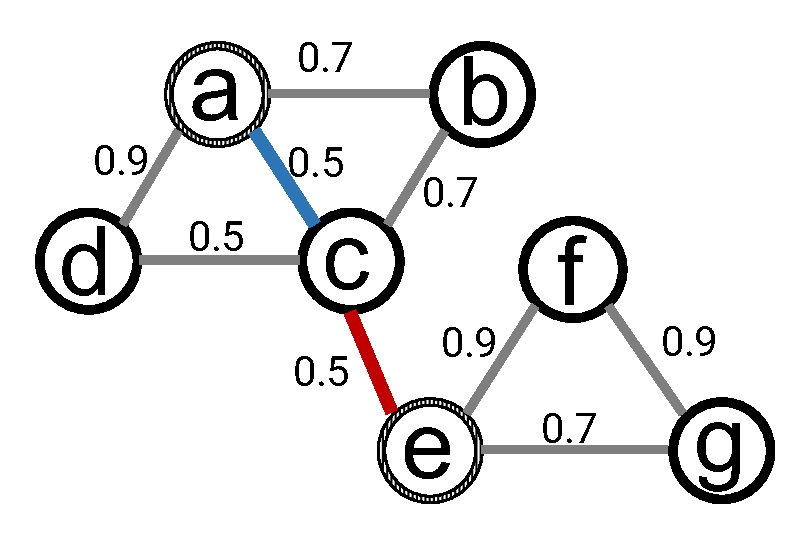
\includegraphics[height=3cm]{AddFigure/bridgetExample.pdf}
    \end{minipage}
  }
  \subfigure[The reliability $R_{a,e}$ v.s $p(e)$]{\label{fig:edgeRR}  %(22)
    \begin{minipage}[l]{0.5\columnwidth}
      \centering
      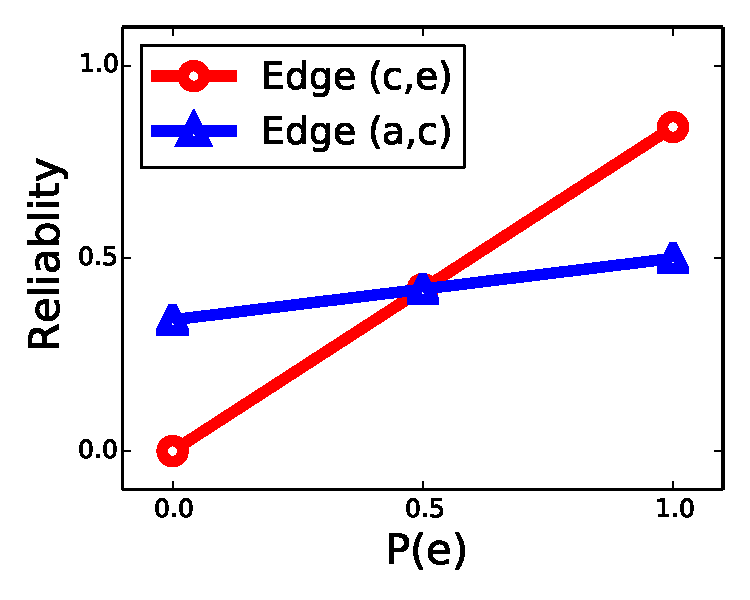
\includegraphics[height=3cm]{AddFigure/ErrExample.pdf}
    \end{minipage}
  }
    \vspace{-1em}
    \caption{(a) Different edges have different effect on the overall graph reliability. (b) Formal {\em Reliability Relevance } measure. A bigger edge's slope indicates  
     big distortion in reliability under small changes to the edge's probability.}
    \vspace{-15pt}
\end{figure}


\textbf{Edge Relevance Analysis.}~~In the context of uncertain graphs, the reliability relevance of edge is defined as reliability discrepancy when one single edge is alterred. Changing a single edge in $\mathcal{G}$ will result in one or more point-wise reliability changing in the corresponding \emph{uncertain} graphs. Thus, the edge reliability relevance is computed as the sum of reliability deviation caused by a single edge alteration. 

\begin{definition} 
  \textbf{Single Edge Reliability Relevance.}~~Given an uncertain graph, the sensitivity of two-terminal reliability $R_{u,v}$ over edge $e$ is defined as follows:
  \begin{align*}
    \mathcal{E}RR^{e}_{u,v} = \lim_{h \rightarrow 0 } \frac{R_{u,v}(\mathcal{G'})-R_{u,v}(\mathcal{G})}{h}
  \end{align*}
  where $\mathcal{G'}$ are identical to the original graph expect the edge $e$ with modified probability $p(e)+h$.
\end{definition}


\begin{lemma}
    \textbf{Factorization Lemma}~~Given an uncertain graph $\mathcal{G}$, the reliability of the node pair $(u,v)$, i.e., $R_{u,v}(\mathcal{G})$, can be factorized via a specific uncertain edge $e$ as follows:
    % \begin{equation*}
    \begin{align*}
      R_{u,v}(\mathcal{G}) &= p(e) R_{u,v} (\mathcal{G}_{e}) + (1-p(e)) R_{u,v} (\mathcal{G}_{\bar{e}}) \\
                          & = p(e) \big[ R_{u,v} (\mathcal{G}_{e}) - R_{u,v} (\mathcal{G}_{\bar{e}}) \big] + R_{u,v} (\mathcal{G}_{\bar{e}})
    \end{align*}
    where uncertain graphs $\mathcal{G}_{e}$ and  $\mathcal{G}_{\bar{e}}$ are identical to the original graph $\mathcal{G}$ with the 
    exception that $e$ is certainly present in the former and certainly not present in the later.
    \label{lemma:fac} 
\end{lemma}

Lemma~\ref{lemma:fac} indicates that the \emph{deviation} of $R_{u,v}$ introduced by a specific edge $e$ is \emph{linear} to the amount of edge probability deviation as shown in Figure~\ref{fig:edgeRR}. In other words, the edge reliability relevance $\mathcal{E}RR^{e}_{u,v}$ equals to the difference of $R_{u,v}$ in the corresponding neighbor \emph{uncertain graphs} $\mathcal{G}_{e}$ and $\mathcal{G}_{\bar{e}}$. First, we remind the reader that edge reliability relevance always be positive since all the connected pairs in $\mathcal{G}_{e}$ are guaranteed to be a superset or at least equal to that in $\mathcal{G}_{\bar{e}}$.


By aggregating edge relevance among all the node pairs $\langle u,v \rangle$, we can get the overall {\em reliability relevance} of edge $e$ $\mathcal{E}RR^{e}(\mathcal{G})$ defined as 
\begin{align*}
    \vspace{-1em}
    \mathcal{E}RR^e(\mathcal{G}) &= \sum_{u,v} |\mathcal{E}RR^e_{u,v}(\mathcal{G})| \\
                                 &= \sum_{u,v} |R_{u,v}(\mathcal{G}_{e}) -R_{u,v}(\mathcal{G}_{\bar{e}})| \\  
                                 &= \sum_{u,v} R_{u,v} (\mathcal{G}_{e}) - \sum_{u,v} R_{u,v}(\mathcal{G}_{\bar{e}}) 
\end{align*}
% \vspace{-0.5em}
Note that $\mathcal{E}RR^e$ equals to the difference of the expected number of connected pairs between two uncertain graphs $\mathcal{G}_{e}$ and $\mathcal{G}_{\bar{e}}$.  
In the context of edge relevance, reliability relevance can be seen as generalization of cut-edges, which quantifies the impact of partial edge deletion or addition on the connectivity in the uncertain graph. 
When the perturbation hits those edges with higher reliability relevance, it would produce bigger structural distortion over the overall \emph{uncertain} graph. 


On the basis of these edge-level reliablity relevance, we can now compute a vertex-level reliability relevance of a given vertex (Say $u$) as a weighted sum of reliability relevance of $u$'s edges $\mathtt{E}^{u}$.  
Fix $u \in \mathcal{G}$ and let $\mathtt{E}^{u}$ be the pairs of vertices that include $v$, we have 
\begin{equation*}
    \vspace{-0.5em}
    \mathcal{V}RR^{u}(\mathcal{G})=\sum_{e \in \mathtt{E}^{u}} p(e)  \mathcal{E}RR^{e}(\mathcal{G})
    \vspace{0.5em}
\end{equation*}

The $\mathcal{V}RR^{u}(\mathcal{G})$  is a measure of the expected impact of vertex modification on the graph reliability. Namely, the higher the vertex's reliability relevance, the larger reliability distortion introduced by modification associated with its edges.

